% ថ្នាក់ទី ១១ (វិទ្យាសាស្ត្រសង្គម) · ជំពូកទី ១ · មេរៀនទី ៣ · សៀវភៅ ទំព័រ ១៤–២៦
\chapter{ស៊ីតធរណីមាត្រ}

\begin{objBox}[វត្ថុបំណង]
\begin{enumerate}[1]
  \item កំណត់និយមន័យនិងផលធៀបរួមនៃស៊ីតធរណីមាត្រ
  \item កំណត់តួទី $n$ នៃស៊ីតធរណីមាត្រ
  \item បង្ហាញផលគុណតួស្មើចម្ងាយពីតួចុង
  \item គណនាផលបូកតួនៃស៊ីតធរណីមាត្រ
  \item គណនាផលបូកតួនៃស៊ីតធរណីមាត្រអនន្តតួ ។
\end{enumerate}
\end{objBox}

\section{និយមន័យស៊ីតធរណីមាត្រ}

\begin{example}[ឧទាហរណ៍]
គេមានស៊ីត $2, 6, 18, 54, 162, \ldots$ ។ គេបាន
\[
\begin{aligned}
a_1 &= 2\\
a_2 &= 6 = 2 \times 3 = a_1 \times 3\\
a_3 &= 18 = 6 \times 3 = a_2 \times 3\\
a_4 &= 54 = 18 \times 3 = a_3 \times 3\\
a_5 &= 162 = 54 \times 3 = a_4 \times 3 \text{ ។}
\end{aligned}
\]
គេសង្កេតឃើញថា តួនីមួយៗនៃស៊ីត (ក្រៅពីតួទី $1$) ស្មើនឹងតួមុនបន្ទាប់គុណនឹងចំនួនថេរមួយ (ស្មើនឹង $3$) ។ ដូច្នេះ ស៊ីត $2, 6, 18, 54, 162, \ldots$ ហៅថា \textbf{ស៊ីតធរណីមាត្រ} ។ ចំនួនថេរ $3$ ហៅថា \textbf{ផលធៀបរួម}នៃស៊ីតធរណីមាត្រ ។
\end{example}

\begin{definition}
ស៊ីតធរណីមាត្រ គឺជាស៊ីតនៃចំនួនពិតដែលតួនីមួយៗ (ក្រៅពីតួទី $1$) ស្មើនឹងតួមុនបន្ទាប់គុណនឹងចំនួនថេរ $q$ ដែល $q \ne 0$ ។ ចំនួនថេរ $q$ នេះ ហៅថាផលធៀបរួមនៃស៊ីតធរណីមាត្រ ។
\end{definition}

\begin{formulaBox}[ជាទូទៅ]
ផលធៀបរួមនៃស៊ីតធរណីមាត្រ តាងដោយ $q$ ដែល $q \ne 0$ ។
\[
q = \frac{a_2}{a_1} = \frac{a_3}{a_2} = \frac{a_4}{a_3} = \ldots = \frac{a_{n+1}}{a_n} \text{ ។}
\]
\end{formulaBox}

\section{តួទី \texorpdfstring{$n$}{n} នៃស៊ីតធរណីមាត្រ}

\begin{example}[ឧទាហរណ៍]
គេមានស៊ីតធរណីមាត្រ $2, 6, 18, 54, 162, \ldots$ ។ គេបាន
\[
\begin{aligned}
a_1 &= 2\\
a_2 &= 2 \times 3 = a_1 \times 3\\
a_3 &= 18 = 6 \times 3 = 2 \times 3 \times 3 = 2 \times 3^2 = 2 \times 3^{3-1}\\
a_4 &= 54 = 18 \times 3 = 2 \times 3 \times 3 \times 3 = 2 \times 3^3 = 2 \times 3^{4-1}\\
a_5 &= 162 = 54 \times 3 = 2 \times 3 \times 3 \times 3 \times 3 = 2 \times 3^4 = 2 \times 3^{5-1}\\
&\ \,\vdots\\
a_n &= 2 \times \underbrace{3 \times 3 \times \ldots \times 3}_{(n-1) \text{ តួ}} = 2 \times 3^{n-1} \text{ ។}
\end{aligned}
\]
\end{example}

\begin{formulaBox}[ជាទូទៅ]
តួទី $n$ នៃស៊ីតធរណីមាត្រកំណត់ដោយ ៖ $a_n = a_1 \times q^{n-1}$ ។
\end{formulaBox}

\begin{example}[លំហាត់គំរូ ១]
គេមានស៊ីតធរណីមាត្រ $6, 12, 24, 48, \ldots$ ។
\begin{enumerate}[a]
  \item គណនាតួទី $14$
  \item តើចំនួន $384$ ជាតួទីប៉ុន្មាននៃស៊ីត?
\end{enumerate}
\end{example}
\ans
តាងតួទីមួយ $a_1 = 6$ តួទីពីរ $a_2 = 12$ គេបានផលធៀបរួម $q = \dfrac{a_2}{a_1} = \dfrac{12}{6} = 2$ ។
\begin{enumerate}[a]
  \item តួទី $14$ នៃស៊ីតត្រូវនឹង $a_{14}$ ។ តាមរូបមន្ត គេបាន $a_n = 6 \times 2^{n-1}$ នោះ $a_{14} = 6 \times 2^{13} = 6 \times 8192 = 49152$ ។ ដូច្នេះតួទី $14$ គឺ $a_{14} = 49152$ ។
  \item តាមរូបមន្ត $a_n = a_1 \times q^{n-1}$ ដោយ $a_n = 384$ គេបាន
  \[ \begin{gathered} 384 = 6 \times 2^{n-1} \iff 64 = 2^{n-1}\\ \iff 2^6 = 2^{n-1} \iff 6 = n - 1 \Rightarrow n = 7 \end{gathered} \]
  ដូច្នេះចំនួន $384$ ជាតួទី $7$ នៃស៊ីត ។
\end{enumerate}

\begin{example}[លំហាត់គំរូ ២]
ប្រជាជននៅទីក្រុងមួយមានចំនួន $2$ លាននាក់ក្នុងឆ្នាំ $2000$ ហើយមានកំណើន $4\%$ ក្នុងមួយឆ្នាំ ។ បង្ហាញថាចំនួនប្រជាជនប្រចាំឆ្នាំបង្កើតបានជាស៊ីតធរណីមាត្រ និងព្យាករទុកនូវចំនួនប្រជាជនក្នុងឆ្នាំ $2009$ ។
\end{example}
\ans
តាងចំនួនប្រជាជនក្នុងឆ្នាំ $2000$ ដោយ $a_1 = 2$ លាននាក់ នោះចំនួនប្រជាជនក្នុងឆ្នាំ $2001$ នឹងមាន $2 + 2(0.04) = 2(1.04)$ លាននាក់ ។

ចំនួនប្រជាជនក្នុងឆ្នាំ $2002$ នឹងមាន $a_3 = 2(1.04)^2$ លាននាក់ ។

ចំនួនប្រជាជនក្នុងឆ្នាំ $2003$ នឹងមាន $a_4 = 2 \times (1.04)^3$ លាននាក់ ។

ចំនួនប្រជាជនប្រចាំឆ្នាំបង្កើតបានជាស៊ីតធរណីមាត្រ ។ ដូច្នេះ ចំនួនប្រជាជនក្នុងឆ្នាំ $2009$ នឹងមាន $a_{10} = 2 \times (1.04)^9 = 2\,846\,624$ នាក់ ។

\begin{pro}
\begin{enumerate}[1]
  \item គេមានស៊ីតធរណីមាត្រ $3, 12, 48, 192, \ldots$ ។
  \begin{enumerate}[a]
    \item គណនាតួទី $9$ ។
    \item តើចំនួន $12288$ ជាតួទីប៉ុន្មាននៃស៊ីត?
  \end{enumerate}
  \item គ្រួសារមួយសម្រេចចិត្តបើកគណនីសន្សំប្រាក់ជាមុនសម្រាប់ការសិក្សារបស់កូនគាត់ ។ នៅពេលថ្ងៃចាប់កំណើតកូនរបស់គាត់ គាត់បានយកប្រាក់ចំនួន $100\,000$ រៀលទៅផ្ញើនៅធនាគារដោយបានទទួលអត្រាការប្រាក់សមាស $6\%$ ក្នុងមួយឆ្នាំ ។ ធនាគារទូទាត់អត្រាការប្រាក់មួយឆ្នាំម្តង ។
  \begin{enumerate}[a]
    \item កំណត់ចំនួនប្រាក់សរុបនៅរាល់ចុងឆ្នាំនីមួយៗនៃបួនឆ្នាំដំបូង និងកំណត់ចំនួនប្រាក់សរុបនៅចុងឆ្នាំទី $n$ ។
    \item កំណត់ចំនួនប្រាក់សរុបនៅចុងឆ្នាំទី $21$ ។
  \end{enumerate}
\end{enumerate}
\ans
\begin{enumerate}[1]
  \item ក. $a_9 = 196608$ \quad ខ. $a_7 = 12288$ ។
  \item ក. $a_1 = 106000$, $a_2 = 112360$, $a_3 = 119101.6$, $a_4 = 126247.696$, $a_n = 100000\left(1 + \dfrac{6}{100}\right)^n$\\
  ខ. $a_{21} = 339956.36$ ។
\end{enumerate}
\end{pro}

\section{ផលគុណតួស្មើចម្ងាយពីតួចុង}

\begin{example}[ឧទាហរណ៍]
គេមានស៊ីតធរណីមាត្រ $a_1, a_2, a_3, a_4, a_5, a_6$ ។ $a_1$ និង $a_6$ ហៅថាតួចុង $a_2$ និង $a_5$ ហើយ $a_3$ និង $a_4$ ហៅថាតួនៅស្មើចម្ងាយពីតួចុង ។

បង្ហាញថា $a_1 \times a_6 = a_2 \times a_5 = a_3 \times a_4$ ។

តាមរូបមន្តតួទី $n$ នៃស៊ីតធរណីមាត្រ $a_n = a_1 \times q^{n-1}$ គេបាន
\[
\begin{aligned}
a_1 \times a_6 &= a_1 \times a_1 \times q^{6-1} = a_1^2 \times q^5 &\quad (1)\\
a_2 \times a_5 &= a_1 \times q \times a_1 \times q^{5-1} = a_1^2 \times q^5 &\quad (2)\\
a_3 \times a_4 &= a_1 \times q^{3-1} \times a_1 \times q^{4-1} = a_1^2 \times q^5 &\quad (3)
\end{aligned}
\]
តាម $(1)$, $(2)$ និង $(3)$ គេបាន $a_1 \times a_6 = a_2 \times a_5 = a_3 \times a_4$ ។
\end{example}

បើ $a_1, a_2, a_3, \ldots, a_p, \ldots, a_{n-p+1}, \ldots, a_{n-2}, a_{n-1}, a_n$ ជាស៊ីតធរណីមាត្រ ។ តួ $a_1$ និង $a_n$ ជាតួចុង ហើយ $a_2$ និង $a_{n-1}$, $a_3$ និង $a_{n-2}$, $\ldots$, $a_p$ និង $a_{n-p+1}$ ជាតួស្មើចម្ងាយពីតួចុង នោះ
\[
a_1 \times a_n = a_2 \times a_{n-1} = a_3 \times a_{n-2} = \ldots = a_p \times a_{n-p+1} \text{ ។}
\]

\begin{formulaBox}[ជាទូទៅ]
ផលគុណតួស្មើចម្ងាយពីតួចុងស្មើនឹងផលគុណតួចុងទាំងពីរ ។ គេកំណត់សរសេរ $a_p \times a_{n-p+1} = a_1 \times a_n$ ។

\textbf{ករណីពិសេស} ៖ បីចំនួនតគ្នា $a, b$ និង $c$ ជាស៊ីតធរណីមាត្រសមមូល $\dfrac{b}{a} = \dfrac{c}{b} = q$ ឬ $a \times c = b^2$ ឬ ($b = \sqrt{a \times c}$ ហៅថា មធ្យមធរណីមាត្រ $a$ និង $c$) ។
\end{formulaBox}

\begin{example}[លំហាត់គំរូ]
គេឱ្យបីចំនួនតគ្នា $a, b$ និង $c$ ជាស៊ីតធរណីមាត្រ ។ បង្ហាញថាបីចំនួនតគ្នា $a^2, b^2$ និង $c^2$ ក៏ជាស៊ីតធរណីមាត្រដែរ ។
\end{example}
\ans
បីចំនួនតគ្នា $a, b$ និង $c$ ជាស៊ីតធរណីមាត្រនោះ $b^2 = a \times c$ ។ លើកអង្គទាំងពីរជាការេ គេបាន $(b^2)^2 = (a \times c)^2 = a^2 \times c^2$ ។

ដូច្នេះ បីចំនួនតគ្នា $a^2, b^2$ និង $c^2$ ជាស៊ីតធរណីមាត្រ ។

\begin{pro}
\begin{enumerate}[a]
  \item តើគេត្រូវបន្ថែមចំនួនប៉ុន្មានទៅលើចំនួន $3, 24, 94$ ដើម្បីឱ្យបីចំនួនតគ្នាជាស៊ីតធរណីមាត្រ?
  \item រកមធ្យមធរណីមាត្រនៃពីរចំនួន $4$ និង $9$ ។
  \item គេឱ្យស៊ីតធរណីមាត្រមួយដែល $a_3 = 4$ និង $a_5 = 36$ ។ គណនា $a_1$ និងផលធៀបរួម $q$ ។
\end{enumerate}
\ans
\begin{enumerate}[a]
  \item ចំនួនត្រូវថែម $x = 6$
  \item $\sqrt{4 \times 9} = 6$
  \item $q = -3$, $a_1 = \frac{4}{9}$ និង $q = 3$, $a_1 = \frac{4}{9}$ ។
\end{enumerate}
\end{pro}

\section{ផលបូក \texorpdfstring{$n$}{n} តួដំបូងនៃស៊ីតធរណីមាត្រ}

\begin{example}[ឧទាហរណ៍]
គណនាផលបូក $7$ តួដំបូងនៃស៊ីតធរណីមាត្រ $1, 2, 4, 8, 16, 32, 64$ ។

តាង $S$ ជាផលបូកស៊ីតធរណីមាត្រដែលមានផលធៀបរួមស្មើនឹង $2$ ។ គេបាន
\[ S = 1 + 2 + 4 + 8 + 16 + 32 + 64 \quad (1) \]
គុណអង្គទាំងពីរនៃ $(1)$ នឹងផលធៀបរួមស្មើ $2$ គេបាន
\[ 2S = 2 + 4 + 8 + 16 + 32 + 64 + 128 \quad (2) \]
យក $(2) - (1)$ គេបាន
\[ \begin{aligned} 2S - S = {}&(2 + 4 + 8 + 16 + 32 + 64 + 128)\\ &- (1 + 2 + 4 + 8 + 16 + 32 + 64) \end{aligned} \]
\[ S = 128 - 1 = 127 \text{ ។} \]
\end{example}

គេអាចយកឧទាហរណ៍ខាងលើ ដើម្បីកំណត់រូបមន្តផលបូក $n$ តួដំបូងនៃស៊ីតធរណីមាត្រ ។ បើគេយក $S_n$ ជាផលបូក $n$ តួដំបូងនៃស៊ីតធរណីមាត្រដែលមានតួទីមួយ $a_1$ និងផលធៀបរួម $q$ នោះ គេបាន
\[
\begin{aligned}
S_n &= a_1 + a_2 + a_3 + \ldots + a_n\\
S_n &= a_1 + a_1 q + a_1 q^2 + \ldots + a_1 q^{n-1} \quad (1)
\end{aligned}
\]
គុណអង្គទាំងពីរនៃ $(1)$ នឹងផលធៀបរួម $q$ គេបាន
\[ qS_n = a_1 q + a_1 q^2 + a_1 q^3 + \ldots + a_1 q^n \quad (2) \]
យក $(2) - (1)$ គេបាន
\[
\begin{aligned}
qS_n - S_n &= (a_1 q + a_1 q^2 + a_1 q^3 + \ldots + a_1 q^n)\\ &\quad - (a_1 + a_1 q + a_1 q^2 + \ldots + a_1 q^{n-1})\\
\iff (q - 1)S_n &= a_1 q^n - a_1 \Rightarrow (q - 1)S_n = a_1(q^n - 1)
\end{aligned}
\]
បើ $q \ne 1$ គេបាន $S_n = \dfrac{a_1(q^n - 1)}{q - 1}$ ។

\begin{formulaBox}[ជាទូទៅ]
ផលបូក $n$ តួដំបូងនៃស៊ីតធរណីមាត្រដែលមានតួទីមួយ $a_1$ និងផលធៀបរួម $q$ ដែល $q \ne 1$ ស្មើនឹង
\[ S_n = \frac{a_1(q^n - 1)}{q - 1} \text{ ។} \]
\end{formulaBox}

\begin{example}[លំហាត់គំរូ ១]
\begin{enumerate}[a]
  \item គណនាផលបូក $7$ តួដំបូងនៃស៊ីតធរណីមាត្រ $5 + 10 + 20 + 40 + \ldots$ ។
  \item គណនាផលបូកតួនៃស៊ីតធរណីមាត្រ $2 + 6 + 18 + \ldots + 1458$ ។
\end{enumerate}
\end{example}
\ans
\begin{enumerate}[a]
  \item តាង $S = 5 + 10 + 20 + 40 + \ldots$ ជាផលបូកតួនៃស៊ីតធរណីមាត្រដែលមានតួទី $1$ គឺ $a_1 = 5$ ផលធៀបរួម $q = 2$ ។ តាមរូបមន្ត $S_n = \dfrac{a_1(q^n - 1)}{q - 1}$ ។ បើ $n = 7$ គេបាន
  \[ S_7 = \frac{5(2^7 - 1)}{2 - 1} = 5(128 - 1) = 635 \]
  ដូច្នេះ ផលបូក $7$ តួដំបូងនៃស៊ីតធរណីមាត្រគឺ $635$ ។
  \item តាង $S = 2 + 6 + 18 + \ldots + 1458$ ដែល $a_1 = 2$, $a_n = 1458$ និងផលធៀបរួម $q = 3$ ។ តាមរូបមន្តតួទី $n$ គេបាន
  \[ \begin{gathered} a_n = a_1 q^{n-1},\ 1458 = 2 \times 3^{n-1},\ 729 = 3^{n-1},\\ 3^6 = 3^{n-1},\ 6 = n - 1 \Rightarrow 7 = n \end{gathered} \]
  នោះ $S$ ជាផលបូក $7$ តួដំបូងនៃស៊ីតធរណីមាត្រ ។ តាមរូបមន្ត $S_n = \dfrac{a_1(q^n - 1)}{q - 1}$ គេបាន
  \[ S_7 = \frac{2(3^7 - 1)}{3 - 1} = \frac{2(2187 - 1)}{2} = 2186 \]
  ដូច្នេះ $2 + 6 + 18 + \ldots + 1458 = 2186$ ។
\end{enumerate}

\begin{example}[លំហាត់គំរូ ២]
ស្តេចឥណ្ឌាឈ្មោះស៊ីរ៉ាម បានបញ្ជាឱ្យជាងម្នាក់ធ្វើក្តារចត្រង្គ ហើយសន្យាថានឹងជូនរង្វាន់តាមតម្រូវការនៃជាងនោះចង់បាន ។ ពេលធ្វើរួច ជាងនោះស្នើសុំគ្រាប់ស្រូវទាំងអស់ដែលដាក់ក្នុងក្រឡាចត្រង្គទាំង ហើយរបៀបដាក់មានដូចតទៅ ៖ មួយគ្រាប់ក្នុងក្រឡាទី $1$ ពីរគ្រាប់ក្នុងក្រឡាទី $2$ បួនគ្រាប់ក្នុងក្រឡាទី $3$ ប្រាំបីគ្រាប់ក្នុងក្រឡាទី $4$, $\ldots$, ចំនួនគ្រាប់ស្រូវក្នុងក្រឡាបន្ទាប់មកស្មើនឹងចំនួនគ្រាប់ស្រូវក្រឡាមុនគុណនឹង $2$ ។ គណនាផលបូកនៃគ្រាប់ស្រូវទាំងអស់ដែលត្រូវដាក់លើក្រឡាចត្រង្គទាំង $64$ ក្រឡា ។
\end{example}
\ans
តាមបម្រាប់ចំនួនគ្រាប់ស្រូវដែលដាក់លើក្រឡាចត្រង្គទាំង $64$ ក្រឡាបង្កើតបានជាស៊ីតធរណីមាត្រ $1, 2, 4, 8, \ldots$ ឬ $2^0, 2^1, 2^2, 2^3, \ldots$ ដែលមាន $a_1 = 1$ និងផលធៀបរួម $q = 2$ ។

តាមរូបមន្ត $S_n = \dfrac{a_1(q^n - 1)}{q - 1}$ គេបាន
\[ S_{64} = \frac{1(2^{64} - 1)}{2 - 1} = 2^{64} - 1 = 18\,446\,744\,073\,709\,551\,615 \text{ ។} \]
ដូច្នេះចំនួនគ្រាប់ស្រូវដែលដាក់លើក្រឡាចត្រង្គទាំង $64$ ក្រឡាគឺ $18\,446\,744\,073\,709\,551\,615$ គ្រាប់ ។

គ្រាប់ស្រូវចំនួន $37000$ គ្រាប់ប្រហែល $1\text{ kg}$ នោះស្រូវទម្ងន់ $1\text{ t} \approx 37000000$ គ្រាប់ ។ ដូច្នេះស្រូវដែលដាក់លើក្រឡាចត្រង្គទាំង $64$ ក្រឡាប្រហែល $4986 \times 10^8\text{ t}$ ។ គេដឹងថាទិន្នផលស្រូវប្រចាំឆ្នាំបច្ចុប្បន្នរបស់កម្ពុជាប្រហែល $5 \times 10^6\text{ t}$ ។

\begin{pro}
\begin{enumerate}[1]
  \item គេមានស៊ីតធរណីមាត្រ $6\,;\ 3\,;\ 1.5\,;\ 0.75\,;\ldots$ ។ គណនា
  \begin{enumerate}[a]
    \item តួទី $7$
    \item ផលបូក $7$ តួដំបូងនៃស៊ីតធរណីមាត្រ ។
  \end{enumerate}
  \item គណនា $S_n = 7 + 77 + 777 + 7777 + \ldots + \underbrace{77\ldots7}_{n \text{ ដងលេខ } 7}$ ។
  \item លោក $B$ បានដាក់ប្រាក់ $100\$$ ទៅផ្ញើក្នុងគណនីសន្សំនៃធនាគារមួយដោយទទួលបានអត្រាការប្រាក់សមាស $10\$$ ក្នុងមួយឆ្នាំ ។ ធនាគារទូទាត់អត្រាការប្រាក់មួយខែម្តង ។ ប្រាក់សរុបដែលលោក $B$ ទទួលបាននៅចុងឆ្នាំទី $5$ គឺ
  \[ \begin{aligned} A = {}&100 \times \left(1 + \frac{0.10}{12}\right) + 100 \times \left(1 + \frac{0.10}{12}\right)^2\\ &+ 100\left(1 + \frac{0.10}{12}\right)^3 + \ldots + 100\left(1 + \frac{0.10}{12}\right)^{60} \end{aligned} \]
  ។ គណនា $A$ ។
  \item ប៉ោលមួយយោលដំបូងបានប្រវែងធ្នូ $18\text{ cm}$ និងយោលជាបន្តបន្ទាប់មកទៀត ដោយម្តងៗសល់ប្រវែងធ្នូ $95\%$ នៃប្រវែងធ្នូមុន ។
  \begin{enumerate}[a]
    \item កំណត់ប្រវែងធ្នូបន្ទាប់ពីយោលលើកទី $10$ ។
    \item ក្រោយពីយោលបាន $15$ ដង ។ កំណត់ប្រវែងធ្នូសរុបនៃការយោលនោះ ។
  \end{enumerate}
\end{enumerate}
\ans
\begin{enumerate}[1]
  \item ក. $a_7 = \dfrac{3}{32}$ \quad ខ. $S_7 = \dfrac{381}{32}$ ។
  \item $S_n = \dfrac{7}{81}(10^{n+1} - 9n - 10)$ ។
  \item $A = 7808.23$ ។
  \item ក. $a_{10} = 11.34$ \quad ខ. $S_{15} = 193.21$ ។
\end{enumerate}
\end{pro}

\section{ស៊ីតធរណីមាត្រអនន្តតួ}

\begin{example}[ឧទាហរណ៍]
ពិនិត្យស៊ីតធរណីមាត្រអនន្តតួ $18 + 1.8 + 0.18 + 0.018 + 0.0018 + \ldots$ ដែលមានតួទីមួយ $a_1 = 18$ និងផលធៀបរួម $q = \dfrac{1}{10}$ ។ គេបាន
\[
\begin{gathered} S_2 = 19.8,\quad S_3 = 19.98,\quad S_4 = 19.998,\quad S_5 = 19.9998,\\ S_6 = 19.99998,\ \ldots,\ S_n = 19.999\ldots998 \end{gathered}
\]
ដូច្នេះ $S_n$ ខិតជិត $20$ កាលណា $n$ ខិតជិតអនន្ត ។
\end{example}

ពិនិត្យផលបូកស៊ីតធរណីមាត្រអនន្តតួ $a_1 + a_1 q + a_1 q^2 + \ldots + a_1 q^{n-1} + \ldots$ ដែលមានតួទីមួយ $a_1$ និងផលធៀបរួម $q$ ។ គេបាន
\[
\begin{aligned}
S_1 &= a_1\\
S_2 &= a_1 + a_1 q\\
S_3 &= a_1 + a_1 q + a_1 q^2\\
S_4 &= a_1 + a_1 q + a_1 q^2 + a_1 q^3\\
S_5 &= a_1 + a_1 q + a_1 q^2 + a_1 q^3 + a_1 q^4\\
&\ \,\vdots\\
S_n &= a_1 + a_1 q + a_1 q^2 + a_1 q^3 + \ldots + a_1 q^{n-1}
\end{aligned}
\]
តាមរូបមន្តគេបាន $S_n = \dfrac{a_1(q^n - 1)}{q - 1} = \dfrac{a_1 q^n}{q - 1} - \dfrac{a_1}{q - 1}$, $(q \ne 1)$ ។

បើ $|q| < 1$ នោះ $q^n$ កាន់តែតូចទៅៗ កាលណាចំនួនតួ $n$ កាន់តែធំទៅៗមានន័យថា $q^n \to 0$ ពេល $n \to +\infty$ គេបាន $S_n = 0 - \dfrac{a_1}{q - 1} = \dfrac{a_1}{1 - q}$ ពេល $n \to +\infty$ ។ ដូច្នេះ $S_\infty = \dfrac{a_1}{1 - q}$ ។

\begin{formulaBox}[ជាទូទៅ]
ផលបូកតួនៃស៊ីតធរណីមាត្រអនន្តតួ $a_1 + a_1 q + a_1 q^2 + \ldots + a_1 q^{n-1} + \ldots$ ដែល $|q| < 1$ កំណត់ដោយ $S_\infty = \dfrac{a_1}{1 - q}$ ។
\end{formulaBox}

\begin{note}
បើ $|q| \ge 1$ នោះ $S_\infty$ មិនអាចកំណត់បាន ។
\end{note}

\begin{example}[លំហាត់គំរូ ១]
គណនាផលបូកតួនៃស៊ីតធរណីមាត្រអនន្តតួ $6 + 2 + \dfrac{2}{3} + \dfrac{2}{9} + \ldots$ ។
\end{example}
\ans
$6 + 2 + \frac{2}{3} + \frac{2}{9} + \ldots$ ជាផលបូកតួនៃស៊ីតធរណីមាត្រអនន្តតួដែលមាន $a_1 = 6$, $q = \frac{1}{3}$ ។ តាមរូបមន្ត $S_\infty = \dfrac{a_1}{1 - q}$ គេបាន $S_\infty = \dfrac{6}{1 - \frac{1}{3}} = 9$ ។

\begin{example}[លំហាត់គំរូ ២]
សរសេរចំនួនទសភាគខួប $4.\overline{57}$ ជាចំនួនសនិទានដែលមានទម្រង់ $\dfrac{a}{b}$ ។
\end{example}
\ans
$4.\overline{57} = 4 + 0.57 + 0.0057 + 0.000057 + \ldots$ ចាប់ពីតួទី $2$ ទៅជាផលបូកនៃស៊ីតធរណីមាត្រអនន្តតួដែលមាន $a_1 = 0.57$, $q = \dfrac{1}{100} = 0.01$ ។ តាមរូបមន្ត $S_\infty = \dfrac{a_1}{1 - q}$ គេបាន
\[ 4.\overline{57} = 4 + \frac{0.57}{1 - 0.01} = 4 + \frac{0.57}{0.99} = 4 + \frac{57}{99} = \frac{453}{99} \]
ដូច្នេះ $4.\overline{57} = \dfrac{453}{99}$ ។

\begin{example}[លំហាត់គំរូ ៣]
គេយោលប៉ោលមួយ (ដូចរូបខាងស្តាំ) ។ លើកដំបូងបានធ្នូមួយប្រវែង $24\text{ dm}$ បន្ទាប់មកប្រវែងធ្នូថយចុះ $20\%$ ជាបន្តបន្ទាប់ ។ កំណត់ប្រវែងគន្លងសរុបនៃលំយោលប៉ោលចាប់ពីពេលដំបូងដល់ពេលវាឈប់ ។

\begin{center}
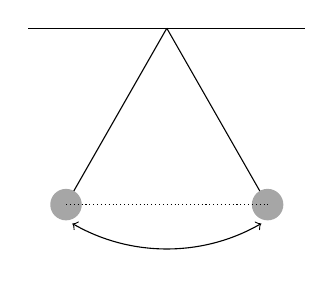
\begin{tikzpicture}[scale=0.8]
  \draw (-2.2,3) -- (2.2,3);
  \draw (0,3) -- (-1.6,0.2) (0,3) -- (1.6,0.2);
  \fill[gray!70] (-1.6,0.2) circle (0.25) (1.6,0.2) circle (0.25);
  \draw[densely dotted] (-1.6,0.2) -- (1.6,0.2);
  \draw[<->] (-1.5,-0.1) arc[start angle=-120,end angle=-60,radius=3];
\end{tikzpicture}
\end{center}
\end{example}
\ans
គេត្រូវកំណត់ផលបូកតួនៃស៊ីតធរណីមាត្រអនន្តតួដែលមានតួទី $1$ គឺ $a_1 = 24$ ហើយផលធៀបរួម $q = 80\%$, $|q| < 1$ ។ តាមរូបមន្តស៊ីតអនន្តតួ $S_\infty = \dfrac{a_1}{1 - q}$ ឬ $S_\infty = \dfrac{24}{1 - 0.8} = 120$ ។

ដូច្នេះប្រវែងគន្លងសរុបនៃលំយោលប៉ោល ពីពេលយោលដំបូងដល់ពេលវាឈប់ស្មើនឹង $120\text{ dm}$ ។

\begin{pro}
\begin{enumerate}[a]
  \item គណនាផលបូកស៊ីតធរណីមាត្រអនន្តតួ $16 + 12 + 9 + \ldots$ ។
  \item សរសេរចំនួនទសភាគខួប $0.\overline{235}$ ជាចំនួនសនិទានដែលមានទម្រង់ $\frac{a}{b}$ ។
\end{enumerate}
\ans
\begin{enumerate}[a]
  \item $S_\infty = 64$
  \item $0.\overline{235} = \dfrac{235}{999}$ ។
\end{enumerate}
\end{pro}

\section*{មេរៀនសង្ខេប ជំពូកទី ១}
\begin{note}[មេរៀនសង្ខេប]
\begin{enumerate}[1]
  \item ស៊ីតនៃចំនួនពិត ជាអនុគមន៍លេខដែលកំណត់ពី $\mathbb{N}$ ទៅ $\mathbb{R}$ ។
  \item ស៊ីតនព្វន្ត ជាស៊ីតនៃចំនួនពិតដែលមានតួនីមួយៗ (ក្រៅពីតួទី $1$) ស្មើនឹងតួមុនបន្ទាប់បូកចំនួនថេរ $d$ មួយ (ហៅថាផលសងរួម $d = a_{n+1} - a_n$) ។
  \item រូបមន្តតួទូទៅនៃស៊ីតនព្វន្ត $a_n = a_1 + (n - 1)\times d$ ។
  \item ផលបូក $n$ តួនៃស៊ីតនព្វន្ត $S_n = \dfrac{(a_1 + a_n)\times n}{2}$ ។
  \item ស៊ីតធរណីមាត្រជាស៊ីតចំនួនពិតដែលតួនីមួយ (ក្រៅពីតួទី $1$) ស្មើនឹងតួមុនបន្ទាប់គុណនឹងចំនួនថេរ $q$ ដែល $q \ne 0$ ។ ចំនួនថេរ $q$ នេះហៅថាផលធៀបរួមស៊ីតធរណីមាត្រ ។
  \item រូបមន្តតួទូទៅនៃស៊ីតធរណីមាត្រ $a_{n+1} = a_n\times q$, $a_n = a_1\times q^{n-1}$ ។
  \item ផលបូក $n$ តួដំបូងនៃស៊ីតធរណីមាត្រ $S_n = \dfrac{a_1(q^n - 1)}{q - 1}$, $(q \ne 1)$ ។
  \item ផលបូកស៊ីតធរណីមាត្រអនន្តតួ $S_\infty = \dfrac{a_1}{1 - q}$, $(|q| < 1)$ ។
\end{enumerate}
\end{note}

\section*{លំហាត់ជំពូកទី ១}
\begin{enumerate}[1]
  \item តួទី $5$ នៃស៊ីតនព្វន្តស្មើ $14$ និងតួទី $12$ ស្មើ $35$ ។ គណនាផលសងរួម តួទី $1$ និងតួទី $n$ ។
  \item ផលបូកនៃ $n$ តួដំបូងនៃស៊ីតមួយកំណត់ដោយ $S_n = n^2 + n$ ។ គណនាតួទី $5$ នៃស៊ីត និងបង្ហាញថាតួនៃស៊ីតនេះជាស៊ីតនព្វន្ត ។
  \item តួទី $3$ នៃស៊ីតធរណីមាត្រស្មើ $3$ និងតួទី $6$ ស្មើនឹង $\dfrac{3}{8}$ ។ គណនាផលធៀបរួមតួទី $1$ និងផលបូក $8$ តួដំបូង ។
  \item គណនា $a$ ដើម្បីឱ្យបីចំនួន $(a - 3)$, $(a + 1)$ និង $(4a - 2)$ ជាបីតួតគ្នានៃស៊ីតធរណីមាត្រ ។
  \item គេឱ្យបួនចំនួនជាស៊ីតធរណីមាត្រ ។ គណនាតួទី $2$ និងទី $3$ នៃស៊ីត បើគេដឹងថាតួទី $1$ ស្មើនឹង $6$ ហើយតួទី $4$ ស្មើនឹង $162$ ។
  \item គេទិញផ្ទះមួយតម្លៃ $30000$ ដុល្លារ ។ អ្នកទិញត្រូវបង់ប្រាក់ជា $6$ ដំណាក់កាលដែលបង្កើតបានជាស៊ីតធរណីមាត្រមានផលធៀបរួម $\dfrac{9}{10}$ ។ កំណត់ប្រាក់ដែលត្រូវបង់តាមដំណាក់កាលនីមួយៗ ។
  \item គេមានស៊ីតនព្វន្ត $(U_n)$ និង $(V_n)$ កំណត់ដោយ $U_1 = 3$ និងផលសងរួមស្មើ $3$ និង $V_1 = 4$ និងផលសងរួមស្មើ $2$ ។
  \begin{enumerate}[a]
    \item កំណត់ $U_n$ និង $V_n$ ជាអនុគមន៍នៃ $n$ ។
    \item គេមានស៊ីត $(W_n)$ កំណត់ដោយ $W_n = \dfrac{U_n}{V_n}$ ។ បង្ហាញថាស៊ីត $(W_n)$ ជាស៊ីតកើន និងកំណត់ $n$ ដើម្បីឱ្យ $W_n - W_{n-1} = \dfrac{1}{28}$ ។
  \end{enumerate}
  \item កំណត់ផលសងរួមនិងតួទីមួយ $U_1$ នៃស៊ីតនព្វន្ត $(U_n)_{n \in \mathbb{N}}$ កើននិងដឹងថា $\begin{cases} U_1^2 + U_2^2 + U_3^2 = 98\\ U_1 - U_2 + U_3 = 4 \end{cases}$ ។ គណនា $U_{10}$ និងផលបូក $10$ តួដំបូងនៃស៊ីត ។
  \item តួដំបូងនៃស៊ីតធរណីមាត្រស្មើ $3$ ហើយមានផលធៀបរួម $r$ ដែលតម្លៃដាច់ខាតនៃ $r$ តូចជាង $1$ ។ ផលបូក $3$ តួដំបូងស្មើ $\dfrac{8}{9}$ នៃផលបូក $6$ តួដំបូង ។ គណនាផលបូកស៊ីតធរណីមាត្រអនន្តតួ ។
  \item \begin{enumerate}[1]
    \item ដោះស្រាយក្នុង $\mathbb{R}$ សមីការ $3x^2 - 8x + 4 = 0$ $(E)$ ។
    \item គេមាន $(U_n)_{n \in \mathbb{N}}$ ជាស៊ីតធរណីមាត្រកើនដែលមាន $U_3$ និង $U_4$ នៃស៊ីតនេះ ជាចម្លើយនៃសមីការ $(E)$ ។ ក. ទាញរកផលធៀបរួមនៃស៊ីតនេះ ។ ខ. គណនាតួទីមួយ $U_1$ នៃស៊ីត ។
  \end{enumerate}
\end{enumerate}

\section*{លំហាត់អនុវត្តន៍}
\begin{enumerate}[1]
  \item កំណត់ផលធៀបរួមនៃស៊ីតធរណីមាត្រ និងសរសេរបួនតួបន្ទាប់ទៀតនៃស៊ីតនីមួយៗ ។
  \begin{tasks}(2)
    \task $4, 20, 100, 500, \ldots$
    \task $\sqrt{2}, 2, 2\sqrt{2}, 4, \ldots$ ។
  \end{tasks}
  \item គេមានស៊ីតធរណីមាត្រ $2, 6, 18, 54, \ldots$ ។
  \begin{enumerate}[a]
    \item គណនាតួទី $7$ ។
    \item តើចំនួន $39366$ ជាតួទីប៉ុន្មាននៃស៊ីត?
    \item គណនាផលបូក $15$ តួដំបូងនៃស៊ីតធរណីមាត្រ ។
  \end{enumerate}
  \item កំណត់ចំនួនតួនៃស៊ីតធរណីមាត្រខាងក្រោម ៖
  \begin{tasks}(2)
    \task $1, 2, 4, 8, \ldots, 8192$
    \task $20, 10, 5, \frac{5}{2}, \ldots, \frac{5}{256}$ ។
  \end{tasks}
  \item បង្ហាញថាស៊ីតខាងក្រោមជាស៊ីតធរណីមាត្រដែលមានតួទី $n$ កំណត់ដោយ
  \begin{tasks}(2)
    \task $a_n = 7 \times (3)^{n-1}$
    \task $a_{n+1} = \frac{1}{8} \times (4)^n$ ។
  \end{tasks}
  \item គេឱ្យ $(a_n)$ ជាស៊ីតធរណីមាត្រ បើគេដឹងថា
  \begin{enumerate}[a]
    \item $a_3 = 18$, $a_7 = 1458$ ។ គណនា $q$ និង $a_{10}$ ។
    \item $a_3 = 20$, $a_6 = 1280$ ។ គណនា $q$ និង $a_1$ ។
    \item $a_1 = 3$, $S_3 = 21$ ។ គណនា $q$ និង $S_7$ ។
  \end{enumerate}
  \item គណនាផលបូកស៊ីតធរណីមាត្រខាងក្រោម ៖
  \begin{tasks}(2)
    \task $48 + 24 + 12 + \ldots + \frac{3}{8}$
    \task $\frac{1}{3} + 1 + 3 + \ldots + 6561$
    \task $9 - 6 + 4 - \ldots - \frac{128}{244}$
    \task $1 - \frac{1}{2} + \frac{1}{3^2} - \frac{1}{2^3} + \frac{1}{3^4} - \frac{1}{2^5} + \ldots - \frac{1}{2^{2n-1}} + \frac{1}{3^{2n}}$ ។
  \end{tasks}
  \item គណនាផលបូកស៊ីតធរណីមាត្រអនន្តដែលមាន $a_2 = -9$ និង $a_5 = \dfrac{1}{3}$ ។
  \item គណនាផលធៀបរួមនៃធរណីមាត្រអនន្តដែលមាន $a_1 = 5$ និង $S_\infty = 15$ ។
  \item ផលបូកពីរតួដំបូងនៃស៊ីតធរណីមាត្រស្មើនឹង $9$ និងផលបូកនៃស៊ីតធរណីមាត្រអនន្តតួស្មើនឹង $25$ ។ គណនា $q$ និង $a_1$ បើផលធៀបរួម $q > 0$ ។
  \item សរសេរជាចំនួនសនិទានដែលមានទម្រង់ $\frac{a}{b}$ នូវចំនួនទសភាគខួបខាងក្រោម ៖
  \begin{tasks}(3)
    \task $0.\overline{7}$
    \task $2.\overline{34}$
    \task $0.\overline{452}$ ។
  \end{tasks}
\end{enumerate}
